\chapter{Support des propriétés NULL dans les frames en PGX.}
\section{Introduction}
NULL est l'un des sujets délicats que les programmeurs doivent traiter. Les objets ou valeurs NULL peuvent apparaître partout dans le code, mais la raison principale est d'avoir des valeurs optionnelles, par exemple dans une base de données SQL. Si nous voulons éviter les valeurs NULL, nous devons alors remplir chaque table avec tous les champs existants et fixer les champs ajoutés à une valeur par défaut, ce qui présente de nombreux inconvénients comme l'augmentation de la consommation de mémoire, la difficulté de choisir ces valeurs par défaut, et peut également générer des bugs et des résultats incorrects si ces valeurs magiques par défaut s'avèrent réelles. De nombreuses questions se posent alors, comme par exemple si une valeur est optionnelle et n'est pas fixée par l'utilisateur, que faut-il y mettre à la place ? Comment procéder si l'exécution rencontre un pointeur nul ? Quel est le résultat d'une opération contenant des valeurs NULL ?
\section{Problème en PGX.D}
PGX.D ne prend pas en charge les valeurs NULL, contrairement à PGX.SM, mais comme nous ne prenons actuellement en charge que les graphes homogènes, cela signifie que tous les sommets/arêtes auront les mêmes propriétés.  C'est pourquoi nous avons utilisé une solution de contournement, qui consiste à avoir des valeurs par défaut au cas où le sommet ou l'arête n'est pas censé avoir cette propriété, ces valeurs par défaut sont choisies avec soin pour conserver l'exactitude des opérations qui les utilisent. Cependant, afin de permettre le support des graphes hétérogènes, où les sommets/arêtes n'ont pas tous les types de propriétés, il sera davantage nécessaire de supporter les valeurs nulles.\\
Par exemple, une requête PGQL sur des graphes homogènes (pas de support des propriétés NULL, mais des valeurs par défaut sont utilisées) donne le résultat suivant:

\begin{figure}[H]  
  \centering
    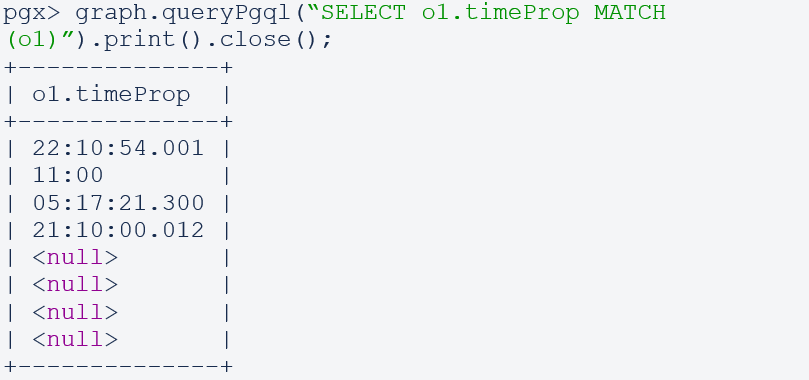
\includegraphics[width=1\textwidth]{chapitre4/Figures/PGXD_query.png}
\end{figure}

En revanche, dans les graphes hétérogènes, avec le support NULL, les valeurs par défaut sont remplacées par "<null>":

\begin{figure}[H]  
  \centering
    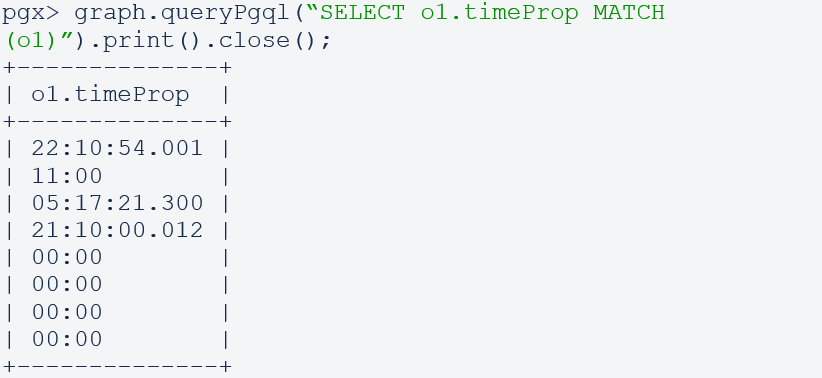
\includegraphics[width=1\textwidth]{chapitre4/Figures/PGX_query.png}
\end{figure}

L'implémentation de NULL n'est pas simple et dépend de beaucoup de facteurs, principalement du langage que vous utilisez et du système que vous implémentez puisque ce dernier peut se soucier ou non de la mémoire et/ou des performances en matière de temps. Dans notre cas, le temps et le rendement de la mémoire sont essentiels, car la charge de travail est énorme et la taille d’un frame peut atteindre des milliards, voire des trillions de lignes.\\

\section{Solution}
Comme nous l'avons déjà dit, les principales préoccupations qui ont motivé nos choix de conception ont été les performances en matière de temps et de mémoire. C'est pourquoi, étant donné la manière dont notre système a été mis en œuvre, nous avons décidé que pour chaque élément, nous ajoutons un indicateur, qui permet de savoir si un élément est NUL ou non. La question qui se pose alors est de savoir quelle structure de données ou quel type de données nous devons utiliser, tel que la modification de ces données, se fera avec un minimum de temps et leur stockage sera aussi minimal que possible.\\
Comme le système est implémenté en C++, l'un des outils les plus faciles à mettre en œuvre et à utiliser est la classe de tableau de bits (std ::bitset)[b.1] de la Standard Template Library (STL), car elle présente les avantages suivants:

\textbf{Avantages :}
\begin{itemize}[label=\textbullet]
\item  Permet une allocation par bits et un accès aléatoire comme un tableau.
\item  Plusieurs méthodes prédéfinies pour le manipuler, comme set(), reset() et flip().
\item  Peut être entièrement mis en cache dans un cache L1 si la taille n'est pas énorme.
\end{itemize}

\textbf{Inconvénients :}
\begin{itemize}[label=\textbullet]
\item  Vous devez connaître la taille de votre ensemble de bits avant la compilation.
\item  Il n'est pas accompagné d'itérateurs, de sorte que la plupart des algorithmes STL ne peuvent pas être utilisés en même temps.
\end{itemize}

Dans notre cas chaque bitset ne consomme que quelques Ko, ce qui le rend un choix idéal, il permettra avec d’autres techniques telle que l’allocation dans la pile en lieux du tas et aussi déclarer les méthodes simples comme inline, d’avoir une implémentation très performante.\\
D’autres considérations qui doivent être prise en charge et le false-sharing comme le système est parallèle cela peut engendrer des pertes de performance et donc chaque bitset doit idéalement être modifié ou consulté que par un seule thread le long du calcule nécessaire.

\newpage
\section{Benchmarking}

Pour justifier notre choix, on devait d'abord évaluer les performances, car c’est une modification critique et va impacter une grande partie du système, puisque pour chaque opération sur un frame, une autre opération liée à des valeurs NULL est également exécutée.

\begin{figure}[H]  
  \centering
    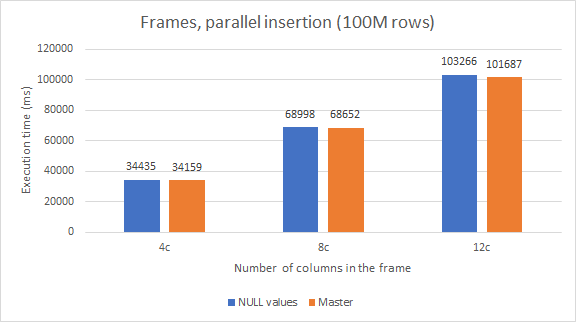
\includegraphics[width=1\textwidth]{chapitre4/Figures/BenchmarkPrallel.png}
  \caption{Benchmark, comparaison entre le temps d'insertion de 100 millions de lignes dans un frame avec et sans support des propriétes NULL}
\end{figure}

\begin{figure}[H]  
  \centering
    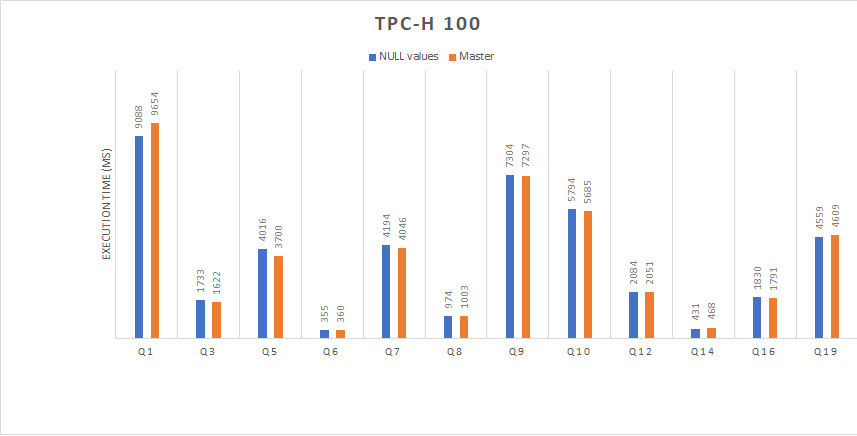
\includegraphics[width=1.1\textwidth]{chapitre4/Figures/BenchmarkTPCH.png}
  \caption{Benchmark TPC-H avec et sans support des propriétes NULL}
\end{figure}

\begin{figure}[H]  
  \centering
    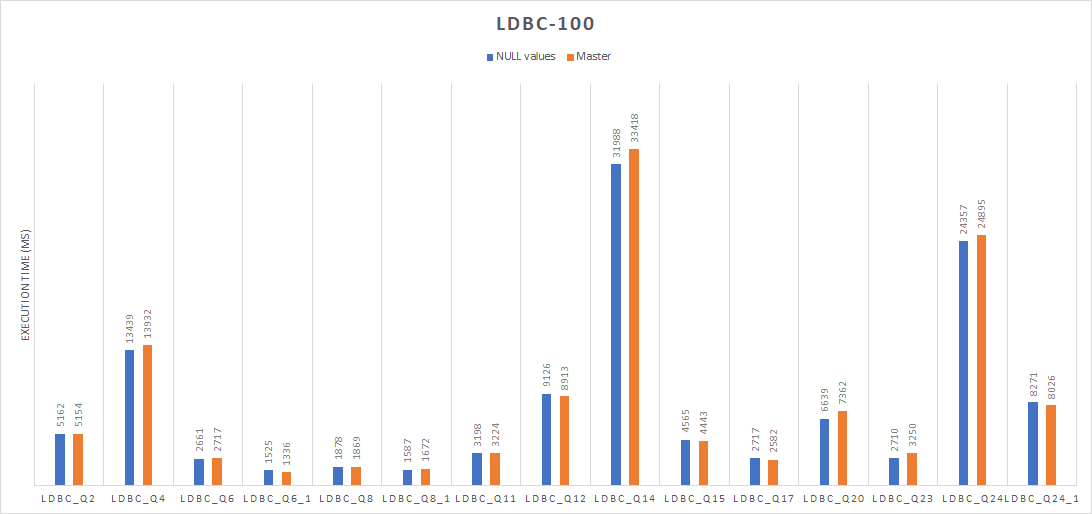
\includegraphics[width=1.1\textwidth]{chapitre4/Figures/BenchmarkLDBC.png}
  \caption{Benchmark LDBC avec et sans support des propriétes NULL}
\end{figure}

\newpage
\section{Conclusion}
Après des évaluations par les pairs et le benchmarking que j’ai réalisé, la conception à étais validé par les membres de l’équipe puisqu’il n’introduit pas un problème de performance considérable.
\begin{itemize}[label=\textbullet]
\item  En mémoire mes modifications on introduit ; 14Mo en mémoire pour un frame de 4 colonnes et 100 millions de rangs.
\item  En matière de temps, les graphiques dans la section précédente montre que mes modifications en introduit une latence négligeable.
\end{itemize}

